\section{Plugins}
\label{implementation:plugins}

Now, we will describe the implementation of a few plugins.
We implemented an infrastructure plugin that can create and remove EC2 instances in Amazon's cloud.
We created a connection plugin that allows the bootware to connect to a remote system via SSH and then execute commands on, or upload files to this system.

\subsection{AWS EC2 Plugin}

This infrastructure plugin allows the bootware to create and remove EC2 instances in Amazon's cloud.
It uses the AWS SDK for Java\footnote{\url{http://aws.amazon.com/sdkforjava/}} to implement this functionality.
This SDK specifies a specific set of action that have to be taken to start an EC2 instance, which we map onto the operations defined by each infrastructure plugin (i.e.: initialize, shutdown, deploy, and undeploy, as described in \autoref{design:plugins}).
\autoref{image:awsplugin} shows a simplified overview of these actions and how they map onto the infrastructure plugin operations.

\begin{figure}[!htbp]
	\centering
	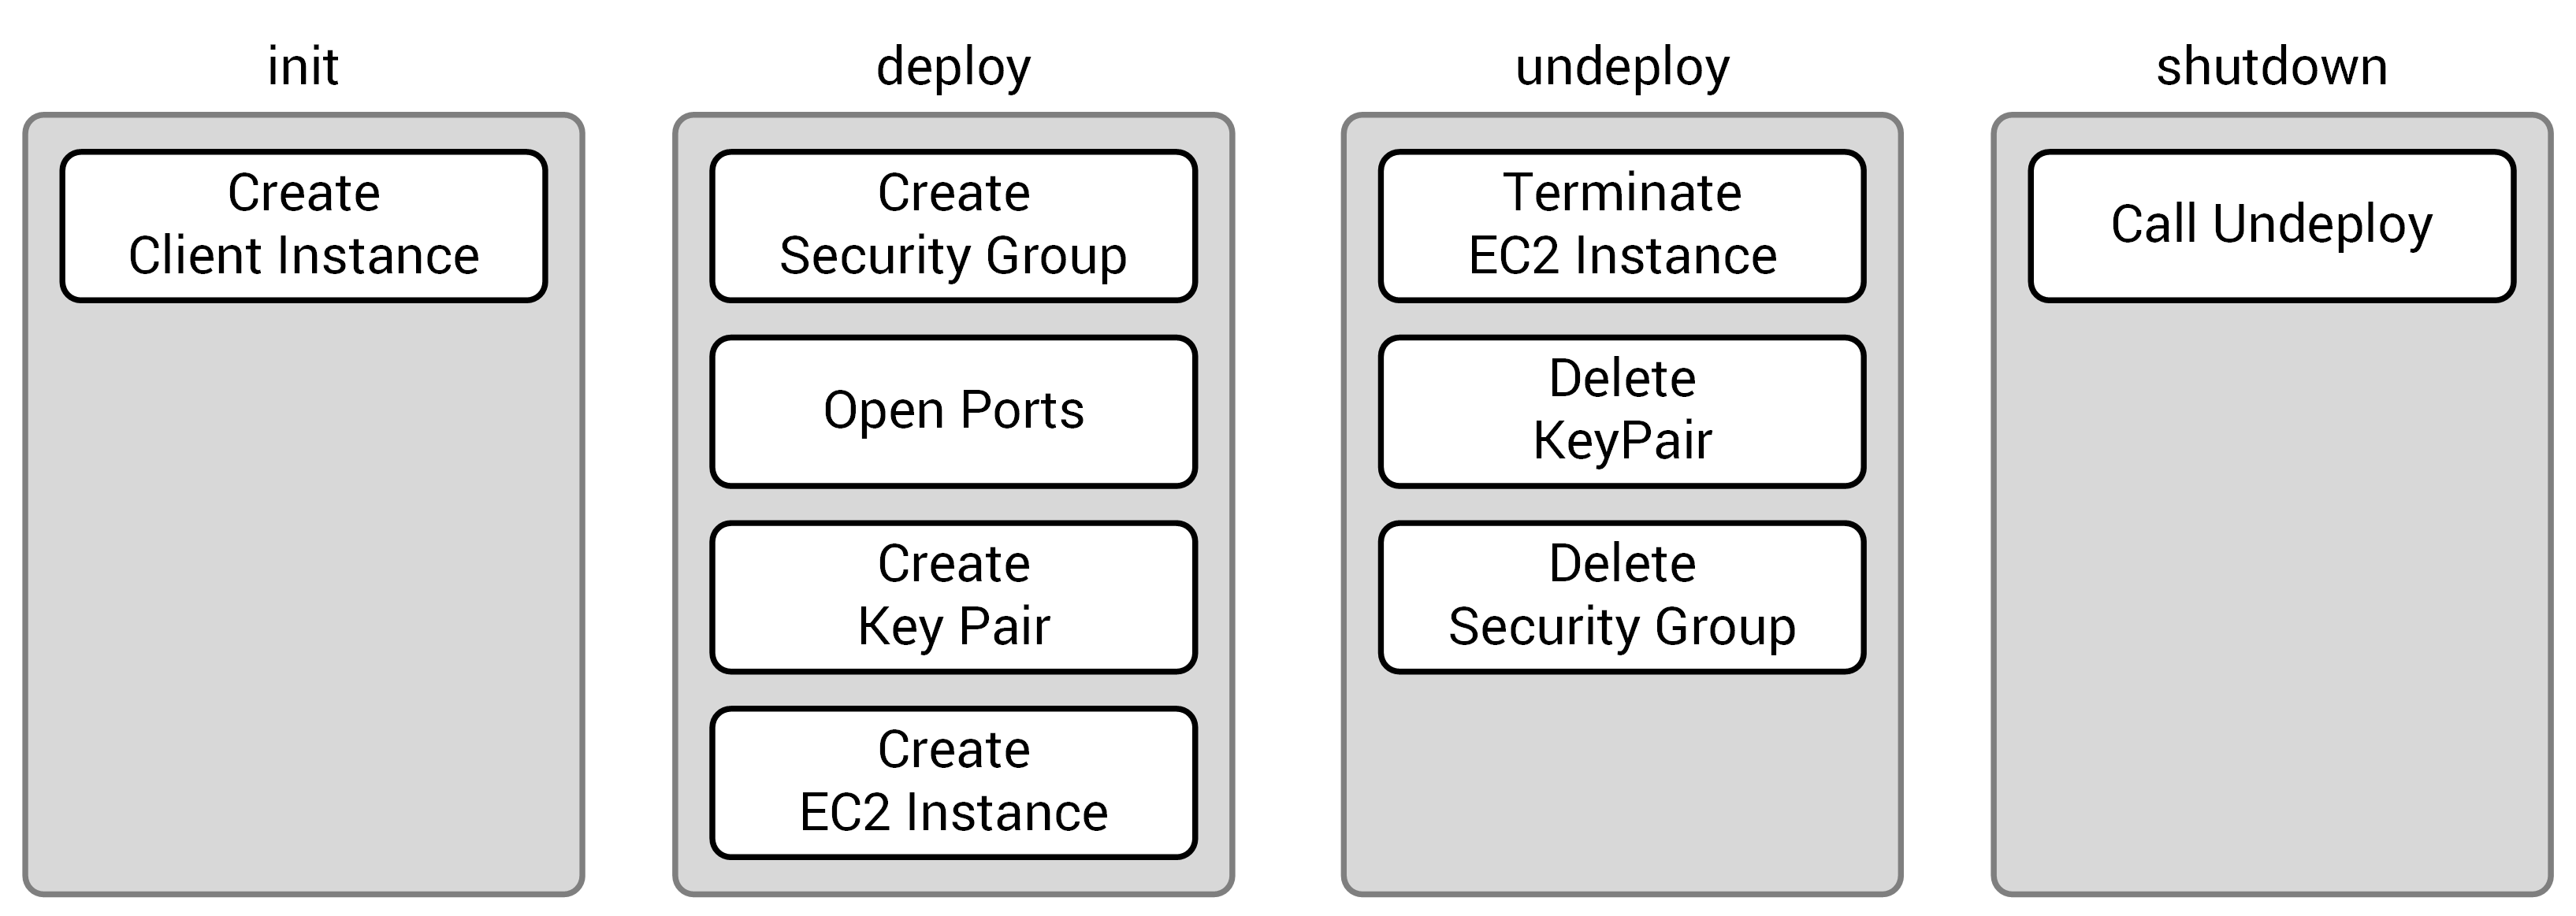
\includegraphics[resolution=600]{implementation/assets/aws_plugin}
	\caption{The operations implemented by the AWS EC2 plugin.}
	\label{image:awsplugin}
\end{figure}

The initialize operation, shown on the left of \autoref{image:awsplugin}, which is called once when the plugin is loaded, creates a client instance, which is an object on which all the following actions will be called.
The client instance is bound to a specific AWS region, which is read from the configuration object that is passed into the initialize operation.

As we can see in the deploy operation in \autoref{image:awsplugin}, we first have to create a security group\footnote{\url{http://docs.aws.amazon.com/AWSEC2/latest/UserGuide/using-network-security.html}}.
Security groups are essentially virtual firewalls that allow or deny traffic to and from all EC2 instances associated with it.
EC2 instances have to be associated with a security group, so we have to create one.
In the next step we open all ports in this security group that we later want to use for communication.
Which ports we open is determined by reading the configuration object.
We also have to create a SSH key pair and retrieve the private key, which we later use when we connect to this EC2 instance via SSH.
In the last step we create the actual EC2 instance.
Once it is up and running, the deploy operation is finished and returns an instance object which contains the URL where the EC2 instance can be reached, as well as the private key for SSH access.

The undeploy operation reverses the deploy operation.
First, it terminates the EC2 instance.
Once the instance is stopped, the key pair and the security group that were created earlier are removed.
We do not have to close the ports we opened, since they are part of the security group and do not exist anymore once the security group is removed.
After this, the EC2 instance created earlier is successfully removed.
There are no further actions necessary during the shutdown operation, but for safety we call the undeploy operation, in case it was not called earlier.

\subsection{SSH Plugin}

This connection plugin allows the bootware to connect to a remote system via SSH.
It uses the Ganymed SSH-2 library\footnote{\url{https://code.google.com/p/ganymed-ssh-2/}}, which implements the SSH-2 protocol in Java.
\autoref{image:sshplugin} shows a simplified overview of the actions necessary to create a SSH connection and how they map onto the connection plugin operations.

\begin{figure}[!htbp]
	\centering
	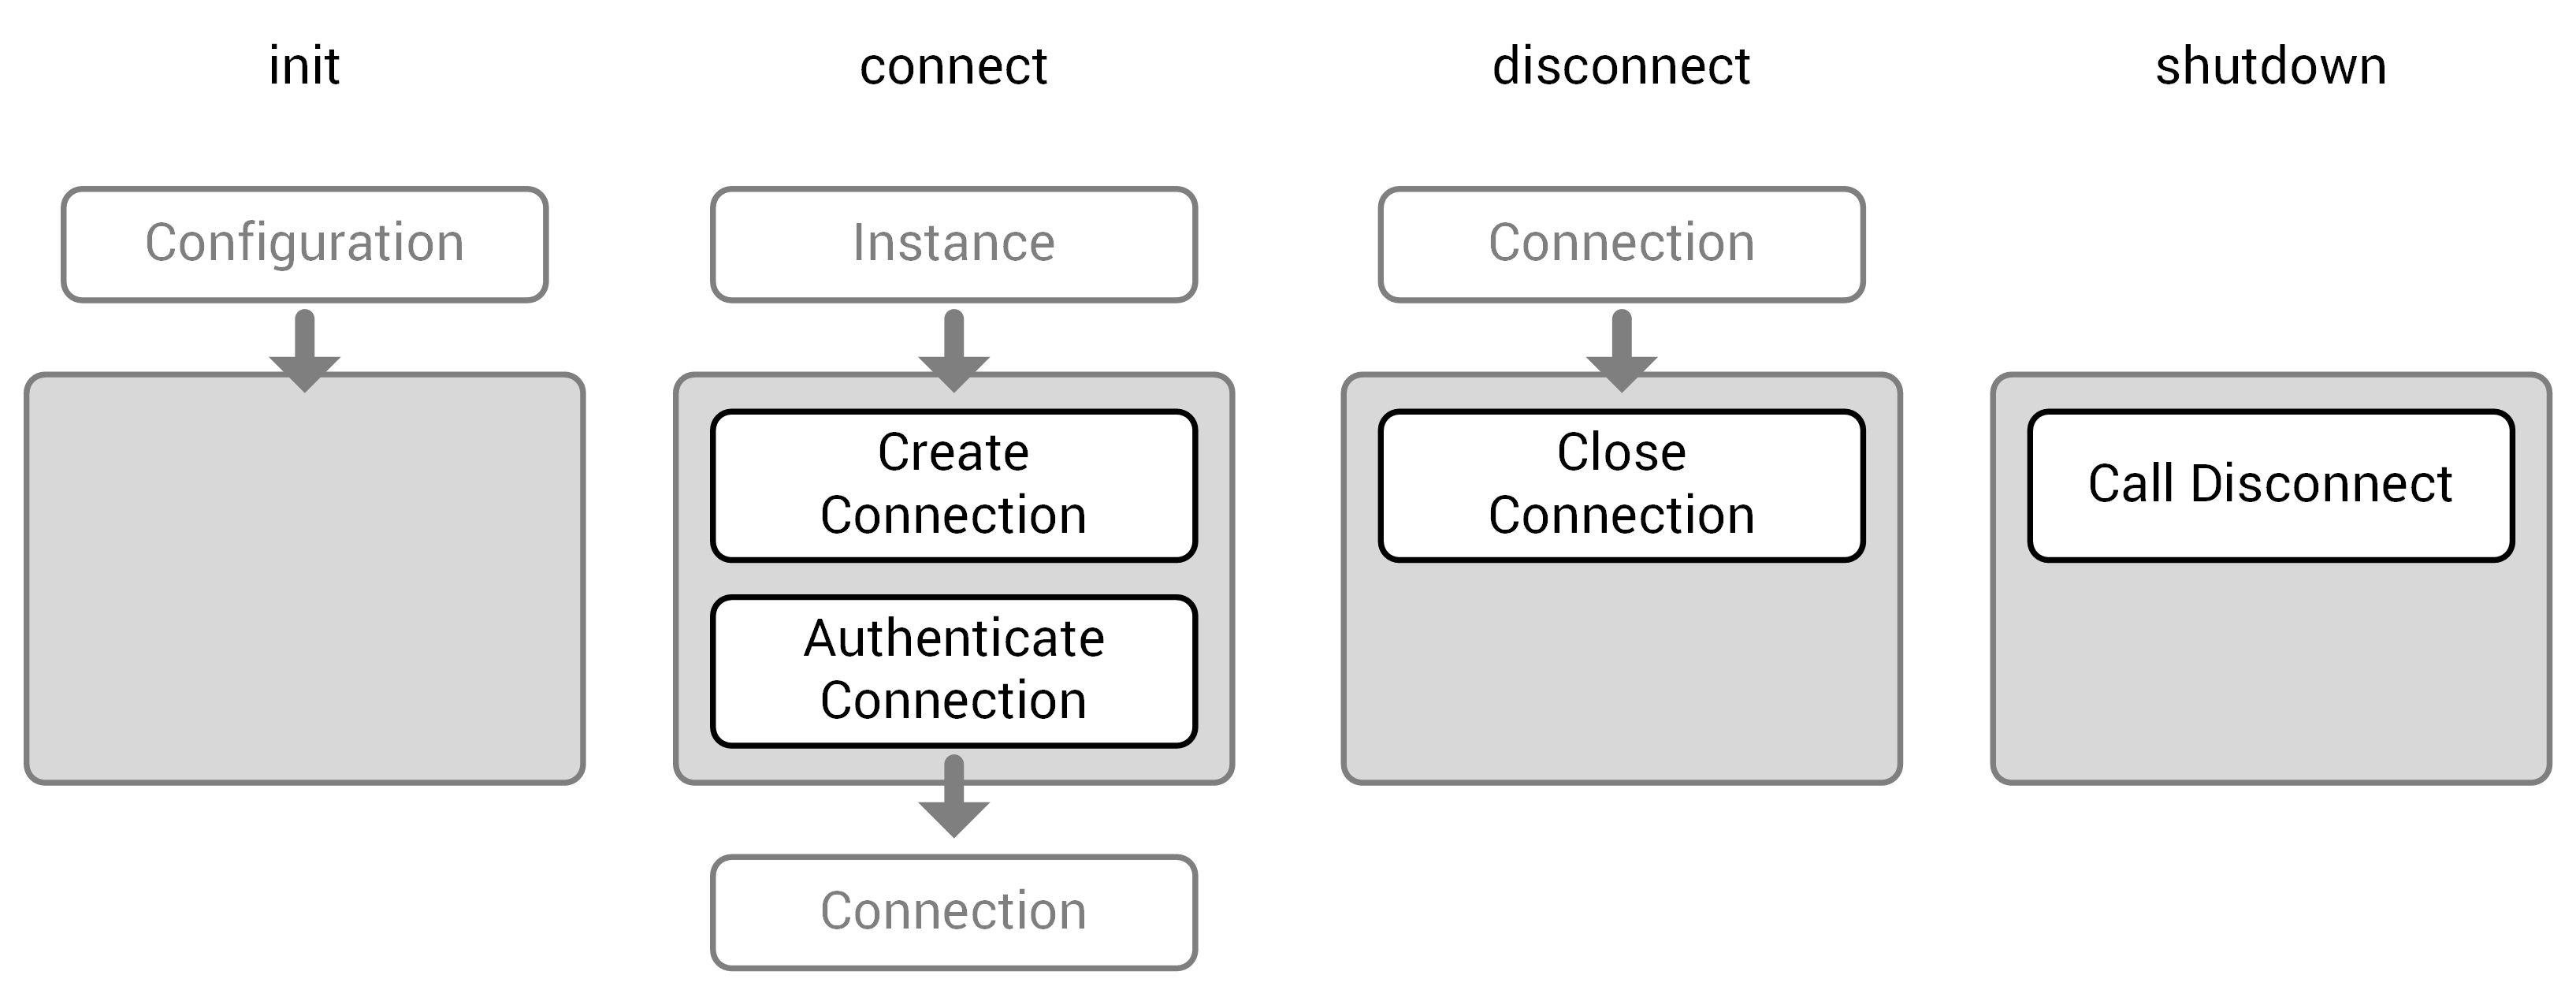
\includegraphics[resolution=600]{implementation/assets/ssh_plugin}
	\caption{The operations implemented by the SSH plugin.}
	\label{image:sshplugin}
\end{figure}

No actions are taken in the initialize operation.
During the connect operation, we first have to create a connection object, which is bound to a certain host name, i.e. the IP address of the remote system that we want to connect to.
We get this address from the instance object passed into the connect operation.
Then, we have to authenticate this connection.
Multiple authentication methods are supported by SSH-2 protocol, including password and public key authentication.
The necessary values for these authentication methods are read from the instance object passed into the connect operation.
Once the connection is authenticated, a connection object is returned, which supports the execute and upload operation that other components can use.

The disconnect operation simply closes the connection associated with the connection object that is passed into it.
The disconnect operation is also called by the shutdown operation at the end of the plugin life cycle to close any connection that might still be open.

\subsection{Remote Bootware Plugin}

This payload plugin allows the local bootware to install the remote bootware on a remote system.
\autoref{image:remotebootwareplugin} shows a simplified overview of the steps involved in the installation of the remote bootware and how they map onto the payload plugin operations.
The undeploy and stop operations where omitted since they are not really required in this case.

\begin{figure}[!htbp]
	\centering
	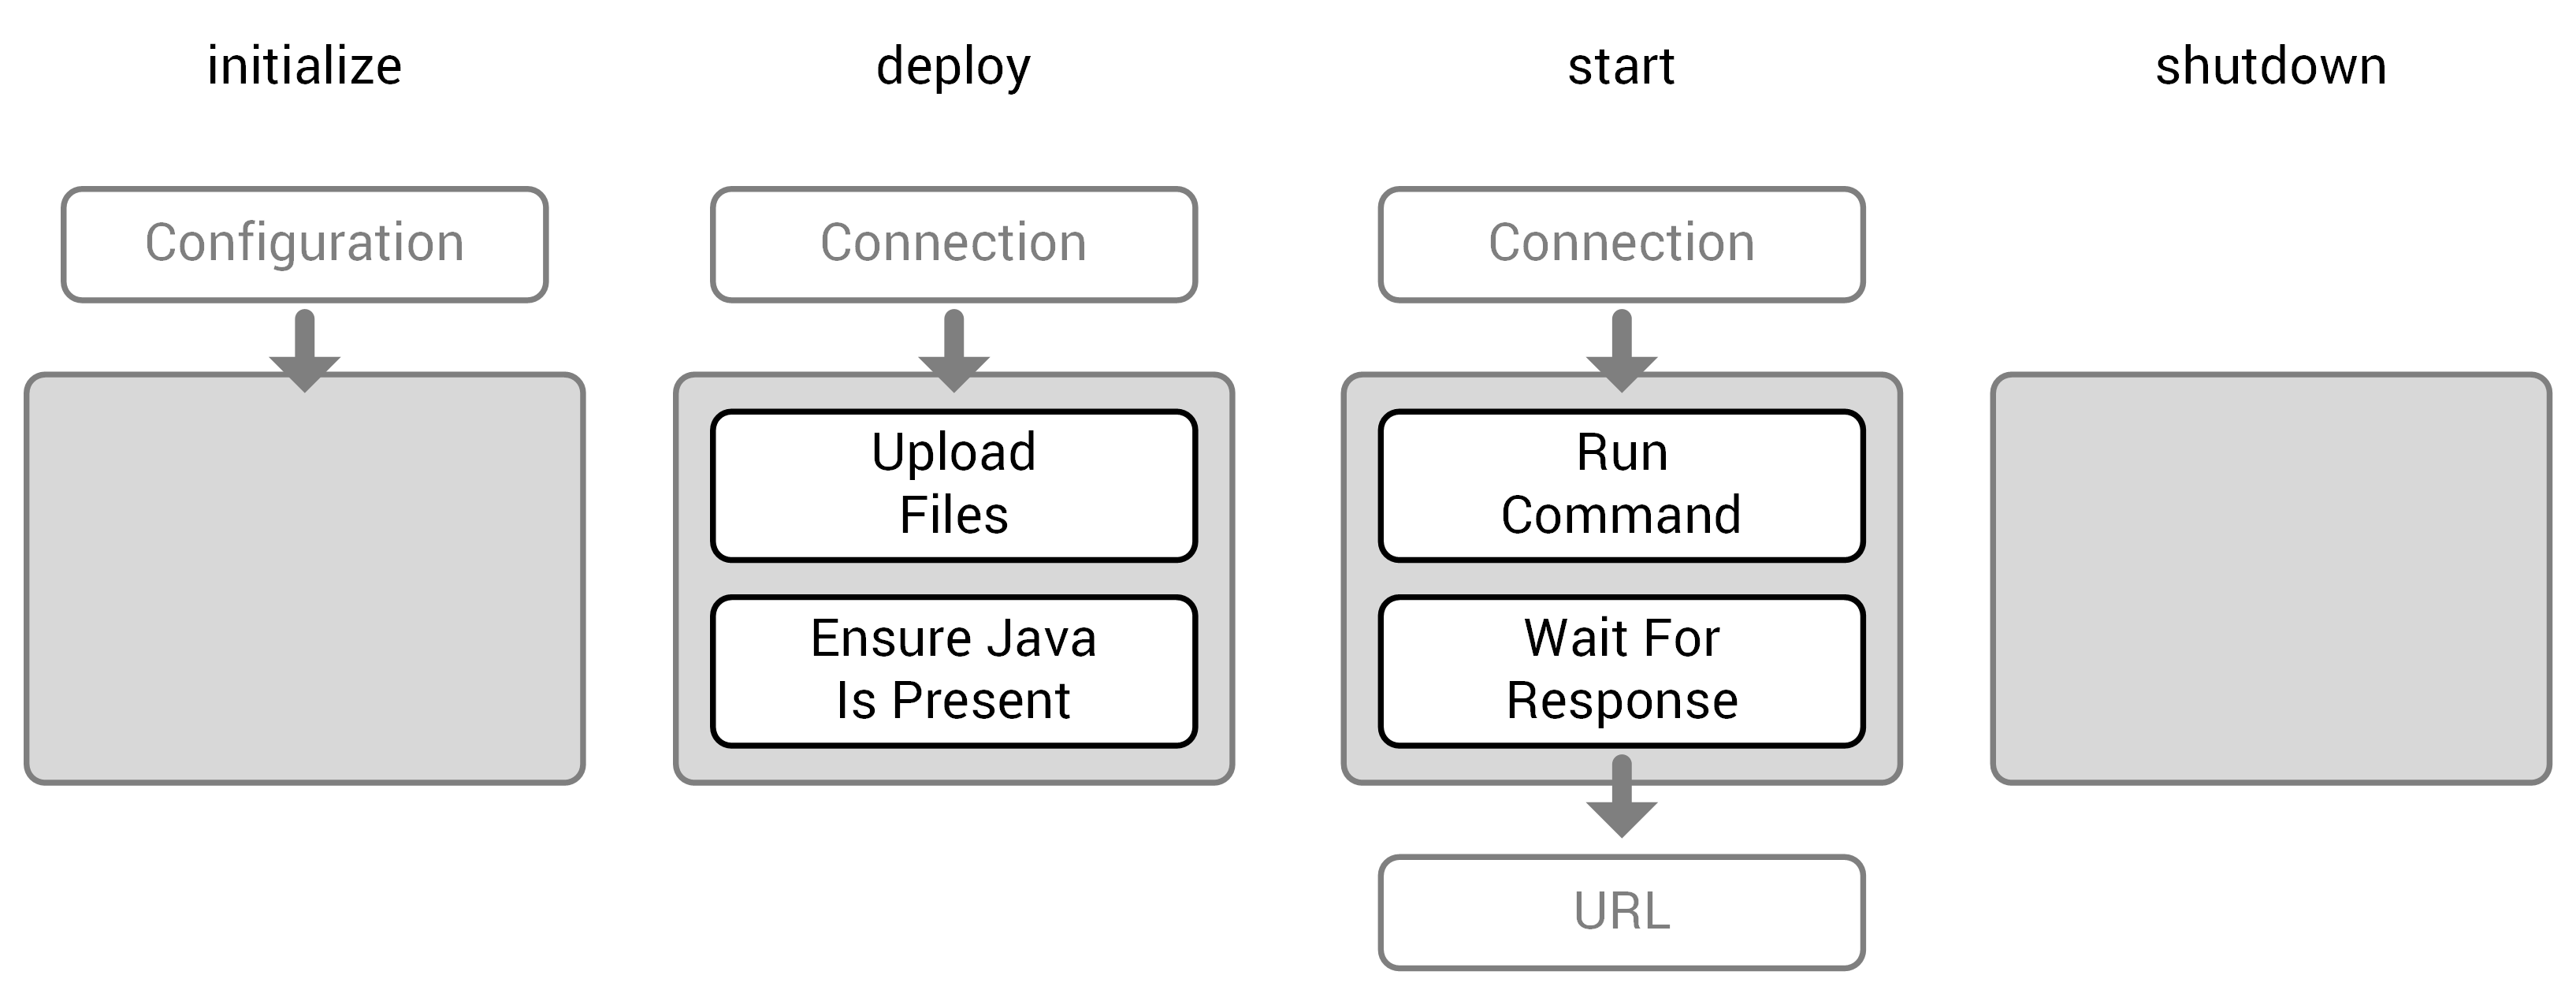
\includegraphics[resolution=600]{implementation/assets/remotebootware_plugin}
	\caption{The operations implemented by the remote bootware plugin.}
	\label{image:remotebootwareplugin}
\end{figure}

In this plugin, the initialize operation does not take any actions.
The deploy operation first uses the operations provided by the connection object it receives as input to upload the remote bootware files from the local to the remote machine.
Then, it checks if the Java version required to execute the remote bootware is present.
If not, it installs the required Java version.
The remote bootware should now be ready to start.
In the start operation a command to execute the remote bootware is send to the remote machine.
Then, the port for the remote bootware web interface is polled until a response is received, which means that the remote bootware should now be ready.
Finally, the URL to the remote bootware is returned.

\subsection{OpenTOSCA Plugin}

This payload plugin allows the bootware to install an OpenTOSCA container on an EC2 instance.
It executes the installation steps described in the OpenTOSCA manual over a connection provided by a connection plugin.
\autoref{image:opentoscaplugin} shows a simplified overview of the steps involved in the installation of OpenTOSCA and how they map onto the payload plugin operations.
The undeploy and stop operations where omitted since they are not really required in this case.

\begin{figure}[!htbp]
	\centering
	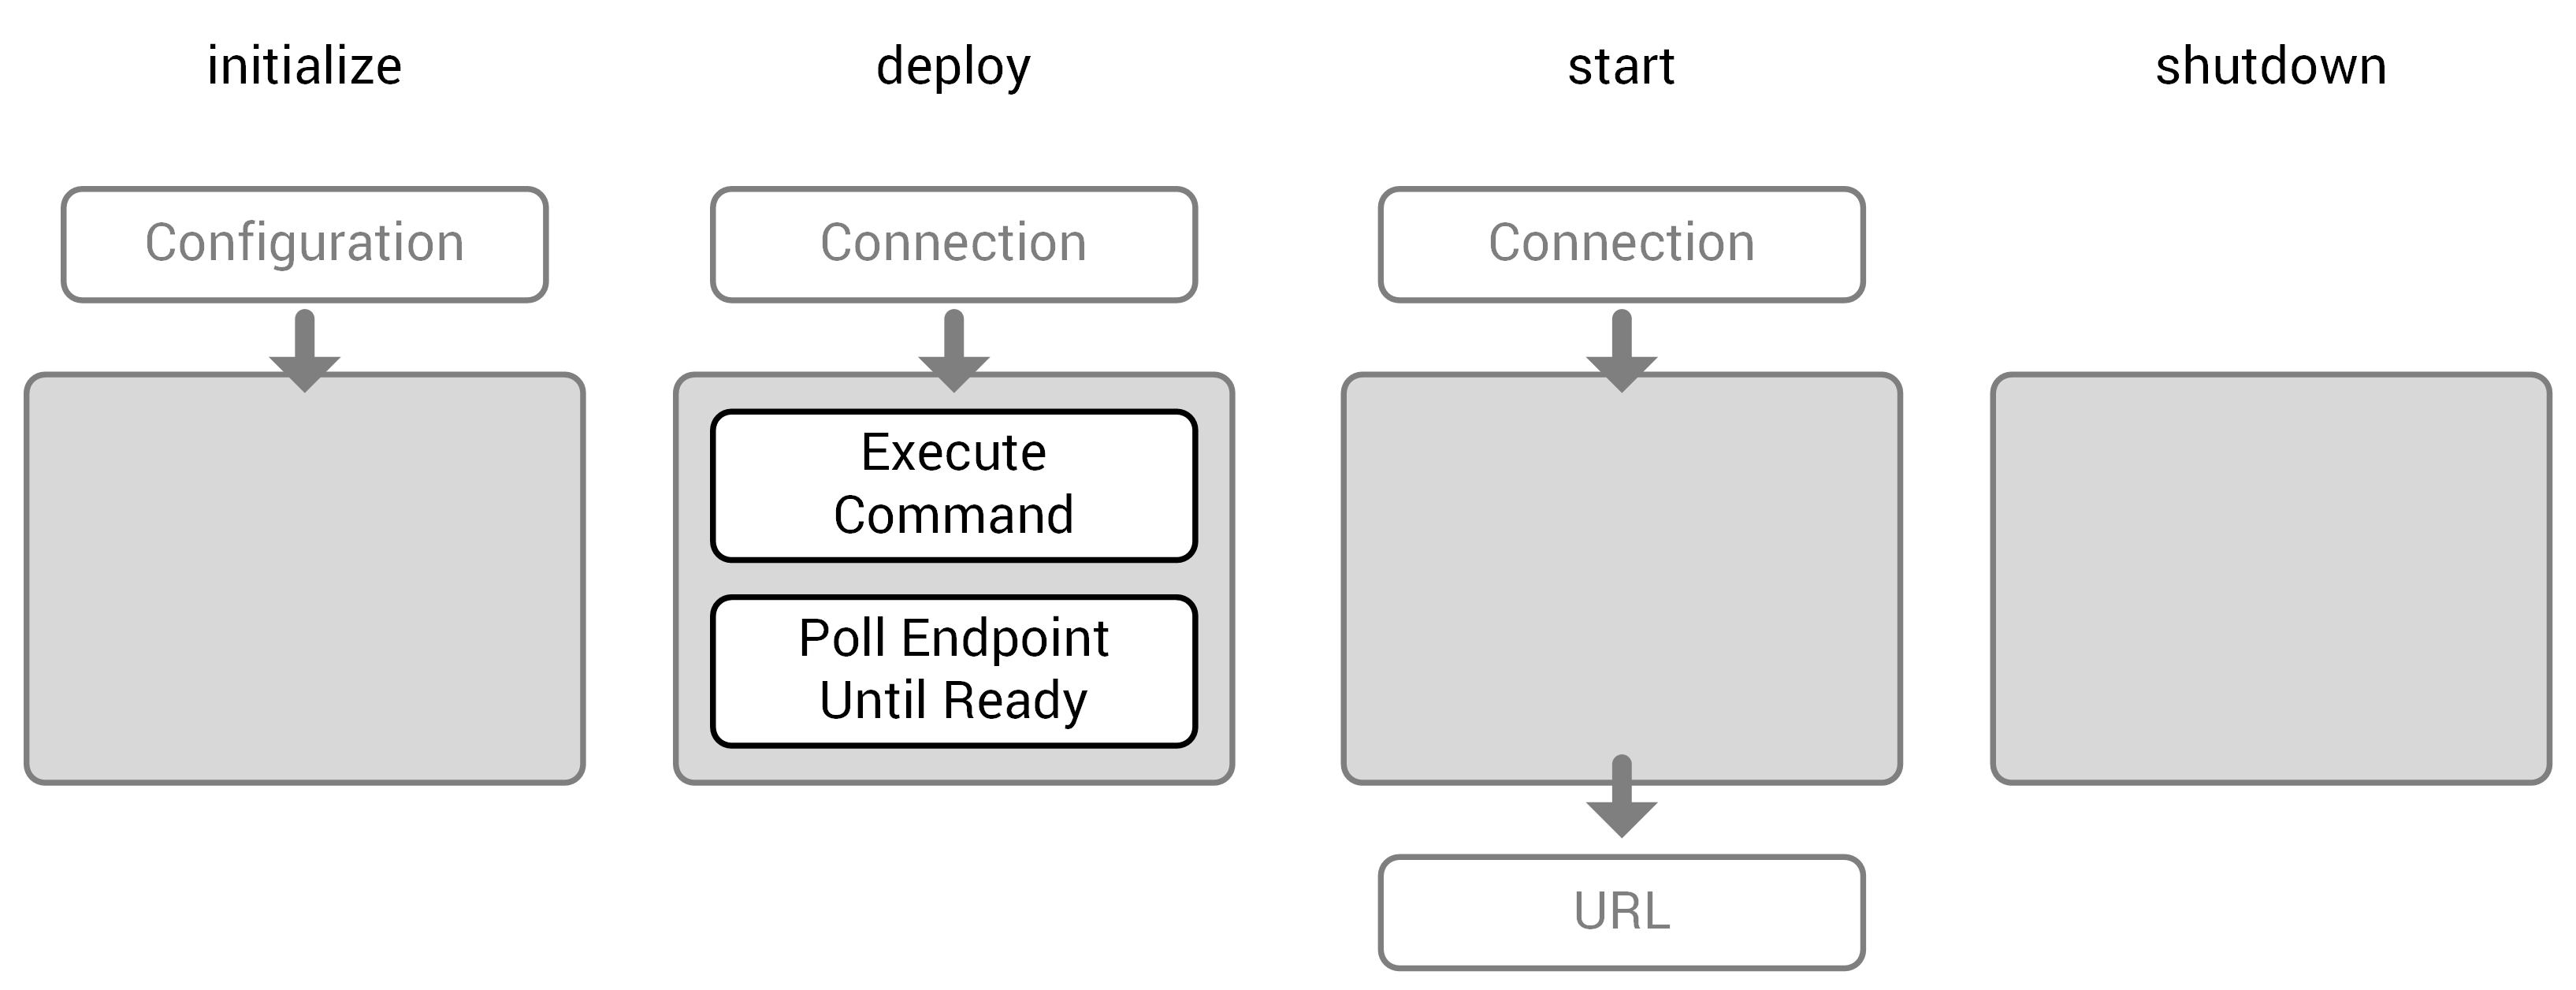
\includegraphics[resolution=600]{implementation/assets/opentosca_plugin}
	\caption{The operations implemented by the OpenTOSCA plugin.}
	\label{image:opentoscaplugin}
\end{figure}

The setup procedure for OpenTOSCA is very simply.
Only one command has to be executed over ssh, which will automatically download and install all necessary components.
After that, port 8080 on the EC2 instance is polled periodically until a connection is possible, which means that the installation process is finished.
The start operation only has to return the URL pointing to the OpenTOSCA instance, since OpenTOSCA was already started by the installation script.

\subsection{File Logger Plugin}

This event plugin logs all events generated by the bootware to a text file.
Unlike the other plugins, it does not implement any other interface operations apart from the standard initialize and shutdown operations.
Rather, it uses event handlers to react to specific events.
\autoref{image:fileloggerplugin} shows a simplified overview of the implementation of this plugin.

\begin{figure}[!htbp]
	\centering
	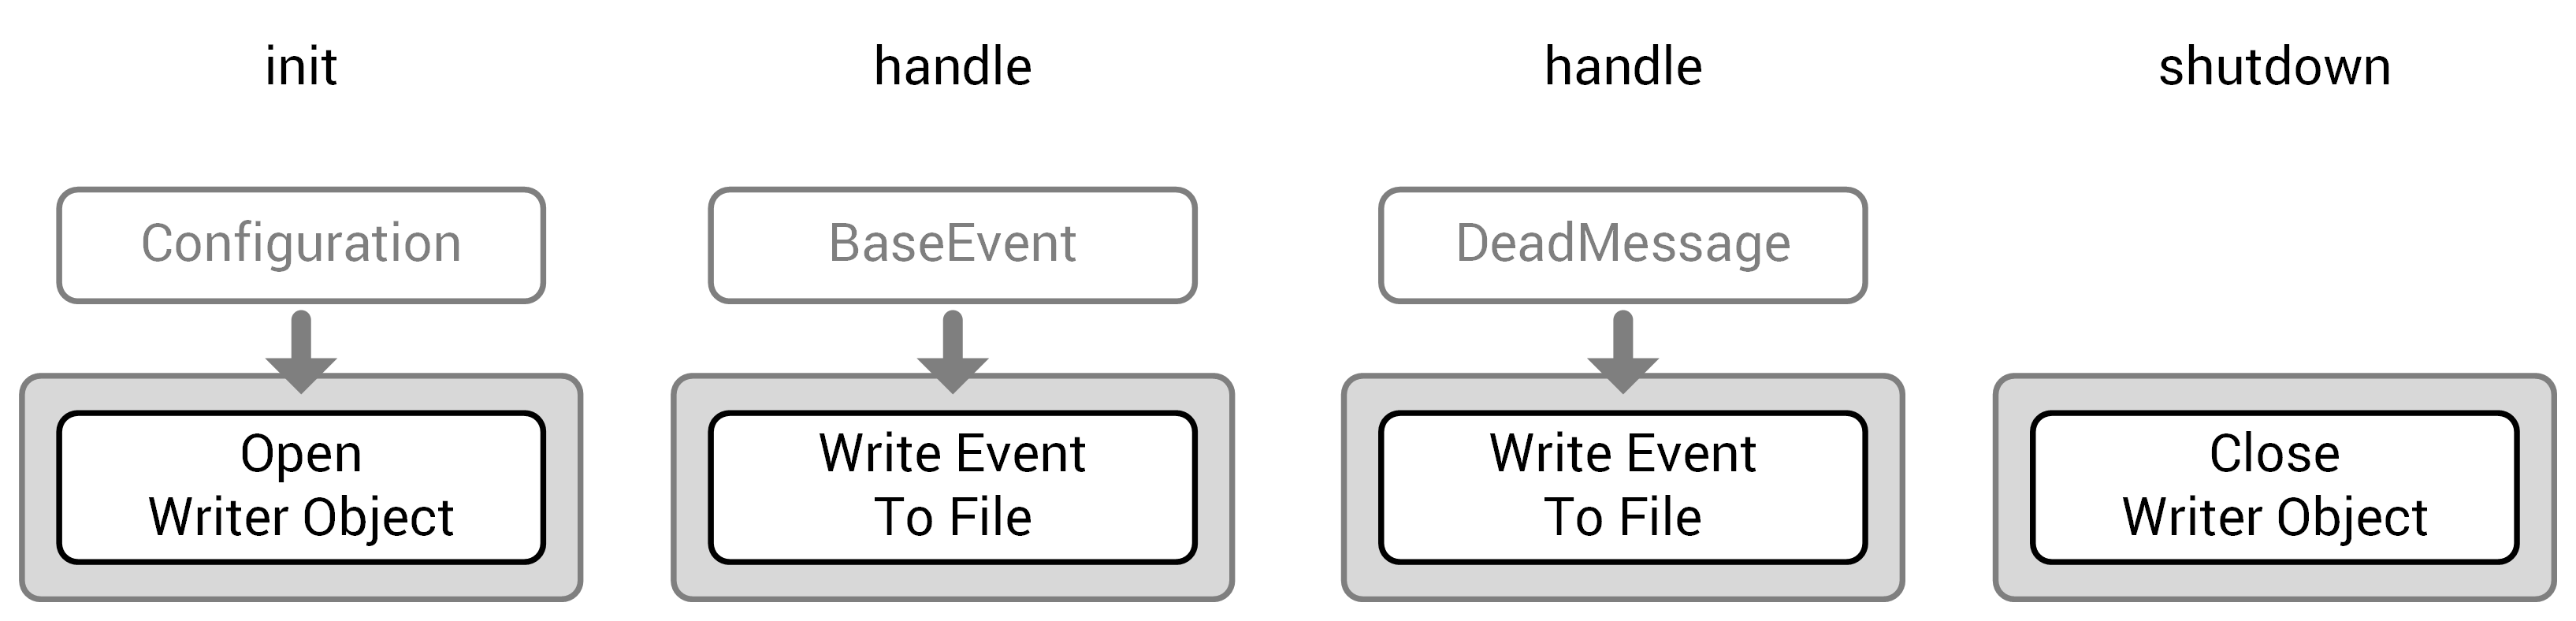
\includegraphics[resolution=600]{implementation/assets/filelogger_plugin}
	\caption{The operations implemented by the file logger plugin.}
	\label{image:fileloggerplugin}
\end{figure}

The initialize operation creates a writer object which opens a text file to write into.
This writer object is then used by the two event handlers shown in the middle to write the events they receive into this file.
The event handler shown on the left reacts to all events of the type BaseEvent, which is the parent event of all events generated by the bootware.
Therefore, it logs any event generated by the bootware into the text file.
The event handler shown on the right reacts to a special DeadMessage event type generated by the PubSub library we use, MBassador.
This event is generated each time an event is published to the event bus to which no one subscribed.
Those events are not received by any listener and are therefor dead.
We log them here for debugging purposes.
The shutdown operation just closes the write object that was created by the initialize operation.
